\documentclass{article}

%Magenes
\textheight = 25cm
\textwidth = 18cm
\topmargin = -2cm
\oddsidemargin=-1cm


%### Hacer uso de símbolos extra ###
\usepackage{latexsym,amsmath,amssymb,amsfonts}

%### Cambio de la fuente del documento###
\usepackage{mathpazo} %palatino

%### Incluir Graphicos ###
\usepackage{graphicx}

%### Comandos especiales para TABLAS ###
\usepackage{multirow, bigstrut}

%### Hiper referencias y ocultando el link (hidelinks) ###
\usepackage[hidelinks]{hyperref}

%##########################################
%Formato archivo.tex, entradas de teclado
%solo dejar uno de los dos archivos activados
\usepackage[utf8]{inputenc}
%\usepackage[latin1]{inputenc}
%###########################################
\usepackage[T1]{fontenc}

%Título
\title{Proyecto Pachamama. Cuestionario \#2}

%Author
\author{Grupo pachamama}
%### Agregar fecha manualmente ###
%\date{mmm, dia, año}

\begin{document}
\maketitle
Nombre del Estudiante:\\

Las siguientes preguntas de éste cuestionario son referentes a la información compartida el viernes 26 de febrero.
Por favor contestar con sus propias palabras y a su manera (para contestar puede hacer dibujos, esquemas mapas, lo que necesite para expresar su idea) No hay restricciones.

\begin{itemize}
		\item [1.] ¿Qué es una entrada? De ejemplos y dibuje el símbolo esquemático. 
		\item [2.] ¿Qué es una salida? De ejemplos y dibuje el símbolo esquemático.
		\item [3.] ¿Qué son conectores? ¿Para qué sirven? Dibuje su símbolo esquemático.
		\item [4.] ¿Qué son las terminales de un elemento?
		\item [5.] ¿Qué son fuentes de energía? De ejemplos.
		\item [6.] La energía se transforma, de ejemplos.
		\item [7.] Se habló de dos formas de corriente eléctrica una directa (DC) y otra alterna (AC), de ejemplos
				de fuentes o elementos donde se puede observar.
		\item [8.] En el circuito de la figura identifique: Entradas, salidas, conectores, drivers, fuentes.
		\item [9.] Explique qué hace el circuito de la figura \ref{1}.
%Imagen para IEEE
%\begin{figure}[hptp]
%    \centering
%    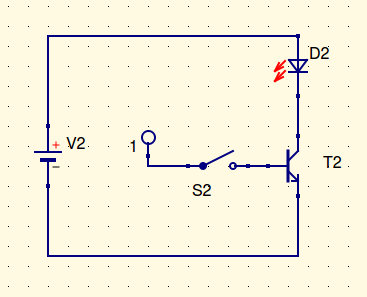
\includegraphics[scale=0.35]{circuito2.png}
%    \caption{Circuito 1.}
%    \label{1}
%\end{figure}
%\smallskip
%		\item [10.] Teniendo en cuenta la respuesta de la pregunta 9, ¿qué sucede en el circuito de la figura \ref{2}?.

%Imagen para IEEE
%\begin{figure}[hptp]
%    \centering
%    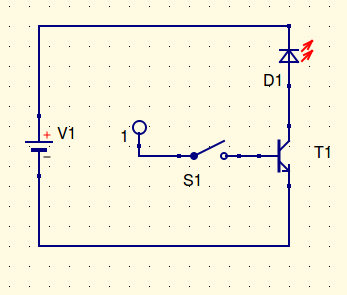
\includegraphics[scale=0.35]{circuito1.png}
%    \caption{Circuito 2.}
%    \label{2}
%\end{figure}
%\smallskip

\end{itemize}

%\include{dir/arch}
\end{document}
